\chapter{Analysis}
	
		
	\section{Verification of problem}\label{sec:verification}
		
 	\subsection{Why a problem?}
 	
 	\subsection{Who says so?}
 	
 	\subsection{Why does it matter?}
 	
\begin{comment}
 	\subsection{Elderly people's approach to technology}
	 	Old people typically will not seek out to use state of the art technology, despite its ability to enable experiences that their age would otherwise prevent. As the elderly retire, they have more time on their hands to do whatever they feel like, and for some of these people gardening could be a very possible interest. But often, age lead to a loss of mobility, limiting old people's ability to garden and their enjoyment thereof, leading to a decrease in life quality. Professional teams have created immersive virtual reality applications like AlohaVR \cite{elderlyVRScout} to help people within the elderly age group seize their issues with chronic pain, relaxation, anxiety, and to provide general entertainment.
	 	%How does the below sentence relate to the above at all? Surely their lack of mobility has nothing to do with their ability to *design* a garden.
	 	So the question could be raised, would it be necessary to have a product that would function for garden designers to work with the elderly and including them in the technological experience? \\
 	
		
		The Pew Research Center has studied the technology adoption of elderly citizens in USA during the last 4 years. They created statistics \cite{seniorTechnology} to show the approach elders to technology as seen in \autoref {fig:oldstats1}. Furthermore the study shows estimates on actual use of different technologies by seniors in the age group 65+ years.
			\begin{figure}[H]
			\centering
			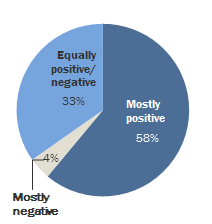
\includegraphics[width=0.4\linewidth]{figure/Analysis/oldpeoplestats1}
			\caption{Elderly peoples approach to technology in society.}
			\label{fig:oldstats1}
			\end{figure} 
		Another statistic shows how large a part of the senior population actually uses Internet and broadband as seen in \autoref{fig:oldstats2}. Nevertheless the graph shows that about 2/3 of the elderly population uses Internet to some extent, which allows the possibility for garden designers to design for the elderly. Furthermore these results creates the chance for garden designers to work with people of all ages, where earlier technology usually would be developed for the use with younger audiences and customers as they were the more common users.
			\begin{figure}[H]
			\centering
			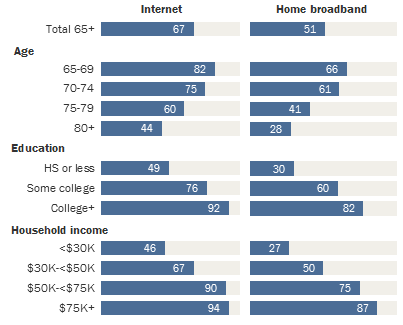
\includegraphics[width=0.6\linewidth]{figure/Analysis/oldpeoplestats2}
			\caption{Elderly peoples use of Internet and Broadband in percent.}
			\label{fig:oldstats2}
		\end{figure} 
	\end{comment}	
	\subsection{Interviews}
	
	The target group had been defined as "Landscape architects working with gardens and particular", and we needed to learn more about this target group. To this end, semi-structured interviews were conducted with different landscape architects. This way we would get a better understanding of both the target group and the context the product would be used in with the customers. The interviews were conducted via telephone and recorded for transcription, translation and analysis. The interview as a qualitative data gathering method, is to be analysed using the coding method to categorize statements from the targets.
	% This section is still usable, but should be rephrased to target the garden designers	
	%Also rewrite to reflect that we never met with the employees	
	
	% when and where
	% what does location and time mean for the data
	
	\subsection{Expert Interviews}\label{sec:expertInterviews}
		For further validation of the problem 4 phone interviews with landscape architects(Experts) were conducted. 2 of the experts were actively using 3D technology for visualizing garden plans for their customers. The other 2 only used sketching by hand to visualize their design for the clients. Due to logistics the interviews were conducted over the phone as the experts had their practises at various locations throughout Denmark. The interviews were semi-structured to allow for new ideas and points to potentially surface. Some practical advantages of interviewing over the phone instead of face-to-face interviews were also considered. These were, amongst others, advantages like Time Efficiency, (Re)arrangement Flexibility and Geographical Reach\cite{telephoneInterview}. 
		
		\subsubsection{Procedure:}This subsection is a brief description of how the interview process was executed.
		
		\paragraph*{Locating experts:}Through online research one project group representative found and e-mailed 12 landscape architects throughout the country and managed to make appointments with 4. During the e-mail correspondence, the experts were informed, and gave their consent on the interviews being recorded and used in the report dependencies in transcribed form.
		
		\paragraph*{Preparation:}
		Through further online research a list of approximately 15-30 questions was compiled. The number depended on whether or not the expert used 3D in his/her practice, as this opened up for further questioning. Here are some examples of the questions:(See appendix \nameref{sec:interviewQuestionsExperts} for the full list)\todo{Update the list in the appendices}

		\begin{itemize}
			\item[-] Do people usually need plans for the entire garden or just parts of it?
			\item[-] Who makes the 3D visualization of the garden? Is it something you create internally in the company, or does it come from outside cooperators? 
			\item[-] How large of a garden area do you usually work with?
			\item[-] Are your clients mostly private or do you also have municipal projects?
		\end{itemize}
		
		\paragraph*{Location:}As previously mentioned the interview were conducted over the phone. The interviewer was placed in a quiet room on campus at Aalborg University Copenhagen and made the phone calls to the experts at the agreed time.

		\paragraph*{Post analysis:}The expert interviews were later transcribed \todo{Insert transcriptions in appendencies and refer to them here} and coded using traditional coding in order to identify patterns and categorize followed by futher analysis of the qualitative data gathered.
		
		\subsubsection{Findings}		
		\todo{More text about the analysis after its done}
		
		\subsubsection{Sub-conclusion}
		\todo{Sub-Conclusion goes here}

	\section{Context}
		
	\section{Target group}\label{sec:targetGroup}
		\subsection{Who are the target }
		
	\section{Technologies}\label{sec:technologies}

		\subsection{Virtual Reality}
			The earliest attempts at a VR experience was in the 1950s\cite{VRS} by Morton Heilig who made the Sensorama\ref{fig:sensorama}; an arcade-style theater cabinet, that featured stereo speakers, stereoscopic 3D display, smell generators, fans and a vibrating chair.
			\begin{figure}[H]
				\centering
				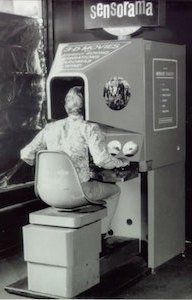
\includegraphics[width=0.4\linewidth]{figure/Analysis/sensorama2}
				\caption{The Sensorama made by Morton Heilig in the 1950s. Fully featured first step at virtual reality.}
				\label{fig:sensorama}
			\end{figure}
			There were a couple of short movies made for the Sensorama, but these were all produced and edited by Morton Heilig himself. The whole setup was stationary, and didn't feature any Head Mounted Display (HMD), so the user had to sit in the vibrating chair and look straight at the display for the duration of the movie. The more modern versions do not include features like smell and fans, but are also geared more towards mobility and full body immersion, and having a vibrating chair doesn't promote that idea.\\
			
			Morton Heilig later went on to further develop the idea of virtual reality, by making the first HMD in form of the Telesphere Mask\cite{VRS} in 1960. This took the immersive nature of his first product to a more personal level, even though it still just were a simple stereoscopic 3D wide view, with stereo sound. It did however look more like the virtual reality headsets of the modern day as seen in \autoref{fig:telesphere}.
			\begin{figure}[H]
				\centering
				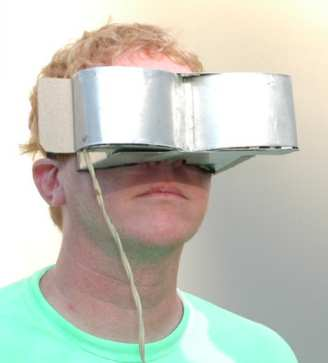
\includegraphics[width=0.25\linewidth]{figure/Analysis/TelesphereMask}
				\caption{The first attempt at HMD virtual reality headset, made by Morton Heilig in 1960. It worked by having stereoscopic 3D vision and stereo sound.}
				\label{fig:telesphere}
			\end{figure}
			Even though it was a step in the direction of a functioning virtual reality headset, it was still only a display showing a movie, it didn't have any motion tracking, or interaction between the user and the movie being watched. There was a sore lack of immersion, which is what makes the virtual reality headsets of today what they are.\\\\

			In 1961 the first motion tracking HMD was developed\cite{VRS}, it was made for military purposes, and was focused on tracking the head movements to control a remote camera. This was to allow a soldier to view remote locations in a natural fashion, without risking the viewer to actually be physically present. It used magnets to accomplish the head motion tracking.\\
			
			After the initial excitement for virtual reality died down with the invent of the world wide web in the mid 90's, the industry waited patiently for hardware that could provide the immersion that tied the experience as a whole together. All of the early attempts had one flaw in common; the hardware couldn't provide close to realistic or good looking graphics at a frame rate that wouldn't induce motion sickness in the user, at a price that a normal consumer could afford\cite{vergeVR}. And hence the virtual reality industry laid dormant until 2013 when a young man called Palmer Luckey created a kickstarter page for a virtual reality headset called Oculus Rift\cite{createOculus}. This headset sparked a wide public interest in virtual reality as a medium, and lead to the development of the current selection of VR headsets available today. The most current iteration of the Oculus Rift is the CV1 - Consumer Version 1. Its biggest competitor is the HTC Vive, a VR headset with similar hardware specifications. \todo{sauce on vive}
			\subsubsection{Standalone VR}
			Oculus Go\footnote{Oculus Go: \url{https://www.oculus.com/go/}} is a virtual reality headset set to launch in the first quarter of 2018. Developed by the firm behind Oculus Rift, the Go shares many features with the Rift. It is designed for virtual reality games, social applications and different kinds of 360 degree experiences. Furthermore, the Go is lightweight with fabrics which increase comfort during long sessions. Unlike the Rift, Oculus Go does not need to be connected to a computer to function, enabling it to be used in new contexts such as outdoors and while traveling. It utilizes a simple controller for navigation and action to allow complex interaction within the featured applications, although it does not feature fully tracked motion control. Another strength the Go brings is the built in spatial audio, which alongside the 2560x1440 pixel display makes the Oculus Go a serious competitor to current mobile VR headsets.   \\
			\begin{figure}[H]
				\centering
				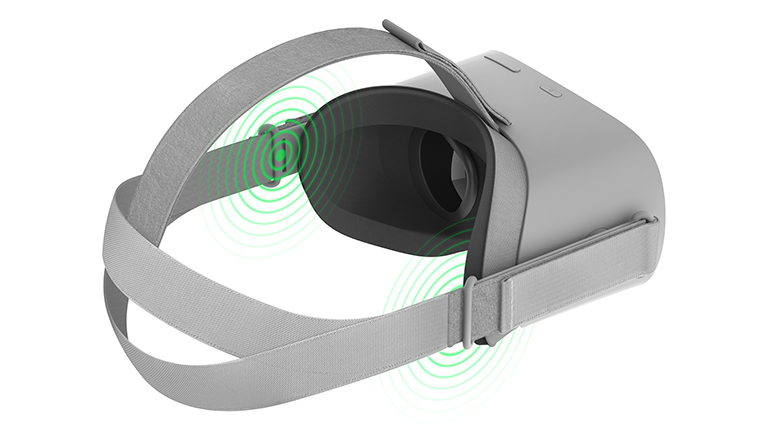
\includegraphics[width=1.0\linewidth]{figure/Analysis/oculusgo}
				\caption{The Oculus Go concept preview}
				\label{fig:Oculus}
			\end{figure}
			
			At the time this report is written, the product is not yet commercially available. Organizations developing for the headset may apply for an early version of the hardware to develop on. It is however possible to develop an application for the Go without owning one, as the Go is directly compatible with applications designed for GearVR. 
			
			Oculus Go is not the only standalone VR headset in the works. Google is working with Lenovo on Daydream, and HTC is developing the Vive Focus, a portable alternative to the HTC Vive. Little information is avaiable about the release date of either product, and the latter is set for a China-exclusive launch. As such, GearVR and Oculus Go are the only current options for portable VR development. \todo{do we need sources here?}
						
			\subsubsection{The essence of VR}
				Virtual reality is a medium\cite{definingVirtualReality}, a medium that has been a long time underway. Starting in the sixties, and being reborn in 2013 by Luckey Palmer, this medium is usually defined by a set of hardware implementations. These hardware implementations range a lot in price and devices, but a broad definition of the medium is:\\

					\begin{quote}
						\textit{Virtual Reality is electronic simulations of environments experienced via head-mounted eye goggles and wired clothing enabling the end user to interact in realistic three-dimensional situations}\cite{coates1992}.\\
					\end{quote}

				This definition is however quite old, being from 1992, but it does still apply to a certain degree to the current state of virtual reality as a device specific medium. Even though the devices, and their capabilities have changed, the way of interaction with the medium is largely the same; Put on a head mounted display, grab the controllers, and explore the 3D world you put yourself into. The rest of the paper will assume the definition of virtual reality as being:\\
				\begin{quote}
					\textit{Virtual Reality is electronic real time simulations of environments experienced via head-mounted eye goggles and one or more controllers enabling the end user to interact in realistic three-dimensional situations}\label{def:virtualRealityDefinition}.\\
				\end{quote}
				 

			\subsection{Fiducial markers}\label{sec:fiducialMarkers}
				By measuring fiducial marker systems, regarding their performance, it is possible to rate the markers by how reliably it finds 
				
				 points matching physical points on the markers. There can be several reasons to why a fiducial marker system would have problems working or live up to the desired performance. This is typically; poor tolerance to lightning conditions and cluttered scenes causing similar markers to be mistaken by each other\cite{fiducialMarkers}. These problems may complicate the system design.\\
				
				There are however a way to figure out if the fiducial marker system is useful and reliable. This can be characterized by some numerical metrics and some qualitative observations, made with carefulness;\\
				\begin{enumerate}
					\item the false positive rate,
					\item the intermarker confusion rate,
					\item the false negative rate,
					\item the minimal marker size,
					\item the vertex jitter characteristics,
					\item the marker library size,
					\item immunity to lighting conditions,
					\item immunity to occlusion,
					\item perspective support,
					\item immunity to photometric calibration, and
					\item the speed performance.\\
				\end{enumerate}
				
				Failing to properly address these criteria will reduce the usability of a marker system remarkably\cite{fiducialMarkers}. All of the numbers have a valid reason for them to be announced; The false positive rate is falsely reporting the presence of a marker when none is present. The intermarker confusion rate is when one marker is mistaken for another. The false negative rate is when the marker can be seen on an image, but not reported. The minimal marker size is the size of the pixels required for the system to detect the marker. The vertex jitter is the noise in the marker corner positions. The library size is the number of unique markers the system is capable of storing. Two important things from the list is immunity to lightning conditions and immunity to occlusion, for a fiducial marker system it is crucial that the system is able to detect and recognize the markers despite the ambient lighting and partial covering of the pattern.\\
				Last is to mention the practical issue of speed performance. A vision-based fiducial marker tracking system must function in real time, using a low cost computing power, for it to be considered useful.\\
				
				All these criteria can be highly fulfilled using a system called ARTag \cite{fiducialARTag}. ARTag consists of a library of patterns with a square border and unique interior digital signature, along with the possibility to detect algorithms found in imagery \cite{fiducialMarkers}.\\
				
				It is important to state here, that not every kind of pattern in a marker is suitable when it comes to fiducial markers\cite{fiducialMarkers}. As an example it is worth mentioning bar codes as seen in \autoref{fig:fiducialmarkers}, these are not suitable as fiducial markers, because they are made to be read by a laser scanner.\\
				Alongside bar codes follows QR. There are two reasons for this; in fiducial marker systems a large field of view is usually preferred. therefore QR is not suitable for this, mainly because they are not intended for this kind of system.This will cause perspective distortion and they will not provide enough image points for 3D pose calculation.The second reason that QR is not suitable is because they require a large area in the image, this will limit the range as to where the markers can be used.\\ 
				
				
					\begin{figure}[H]
						\centering
						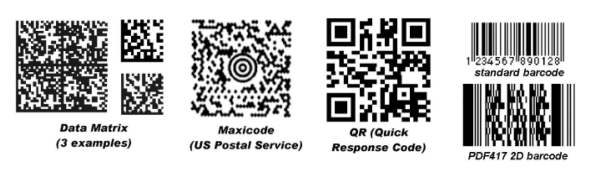
\includegraphics[width=0.9\linewidth]{figure/Analysis/fiducialmarkers.png}
						\caption{Different markers, not suitable for a fiducial marker system.}
						\label{fig:fiducialmarkers}
					\end{figure}
					
				
				As stated above, there are a lot of different markers that can be used for a fiducial marker system, but some are more efficient than others, depending on what kind of system will be used.
				Fiducial marker systems is usually functioning in two different stages; hypothesis generation and verification/identification.\\
				
				To test the pattern, six parameters are still necessary. The perspective projection has to be approximated by a parallel one. For this, a first stage must find candidate regions by locating one or more relatively unique features of the marker this is because the space of possible homographies or parallel transforms is too large to test an image for valid patterns by exhaustive search \cite{fiducialMarkers}.
				A geometric shape or shapes, such as a dot, bar, ellipse, triangle, square, etc., provides an anchor to form a marker detection hypothesis.\\
				
				Moving on to second stage, but with some important notes from stage one, such as; homography or parallel parameters, which checks if the region is actually a marker or just an object in the environment. As prior mentioned regarding coded dot systems, a parallel warp can be calculated on the ellipses major and minor axes.
				as seen in \autoref{fig:fiducialworking}, several marker systems is shown and they all presume planarity and use a parallel or homography mapping.
				
					\begin{figure}[H]
						\centering
						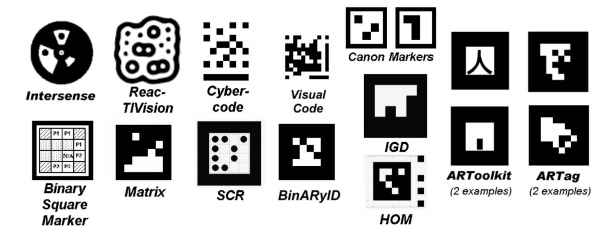
\includegraphics[width=0.9\linewidth]{figure/Analysis/fiducialworking.png}
						\caption{Different markers, suitable for a fiducial marker system.}
						\label{fig:fiducialworking}
					\end{figure}
					
				It is unlikely to find a marker system that does not use any kind of thresholding, connectivity or blob analyses/detection, this is due to details. Though using thresholding and connectivity does not come without some error modes. How well the first stage is implemented affects the false negative detection rate. this is due to incorrect thresholding, which leads to markers that will be missed. Minimal marker size, vertex jitter characteristics, and especially immunity to
				lighting conditions\cite{fidOcclusion} are also something that has to be considered.\\
				
				A system using only parallel mappings will have trouble with larger markers as well as cameras with a small focal length; for example Webcams(in laptops or portable ones) and cameras built into portable devices.
				 
				
				
				
		\subsection{Image Processing}
		
		Image processing is the act of enhancing, or extracting information from, a digital image using certain operations. It will take as input a photograph, computer generated image, or even a video feed, and return an output depending on the operations performed. Visual enhancements could be brightening a scene, increasing color saturation, or resizing, flipping, twisting and turning the image. Information extracted from the frame could be  in the form of counting objects or identifying objects, even complicated ones like faces. 
		
			\subsubsection{Color detection}
			
			One of the simpler things to extract from an image is color. A simple program may count the number of pixels with the RGB color code (255,0,0), which we know as "red". A slightly more sophisticated program will have some leniency built in, counting red-ish colors as being red. This is useful since in a real life scenario, neither the camera nor the light is going to be perfect, and therefore some inaccuracies must be accounted for. 
			
			The ideal color space to use for color detection depends on the specific case. 
			%insert pictures of color spaces
			For example, given the below image of leukocytes (white blood cells) surrounded by other blood cells, which color space would be most suitable for extracting the leukocytes?
			\begin{figure}[H]
				\centering
				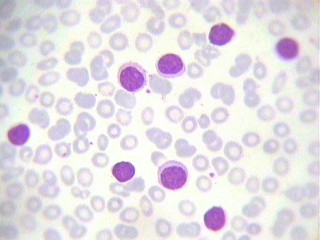
\includegraphics[width=0.2\linewidth]{figure/Analysis/leukocytes.jpg}
				\caption{White blood cells (Purple cells in image)}
				\label{fig:leukocytes}
			\end{figure}
			
			By converting the image to different color spaces and seperating each space into its components, we can see in which channel of which color space the desired objects stand out the most. 
			
					\begin{figure}[H]
				\centering
				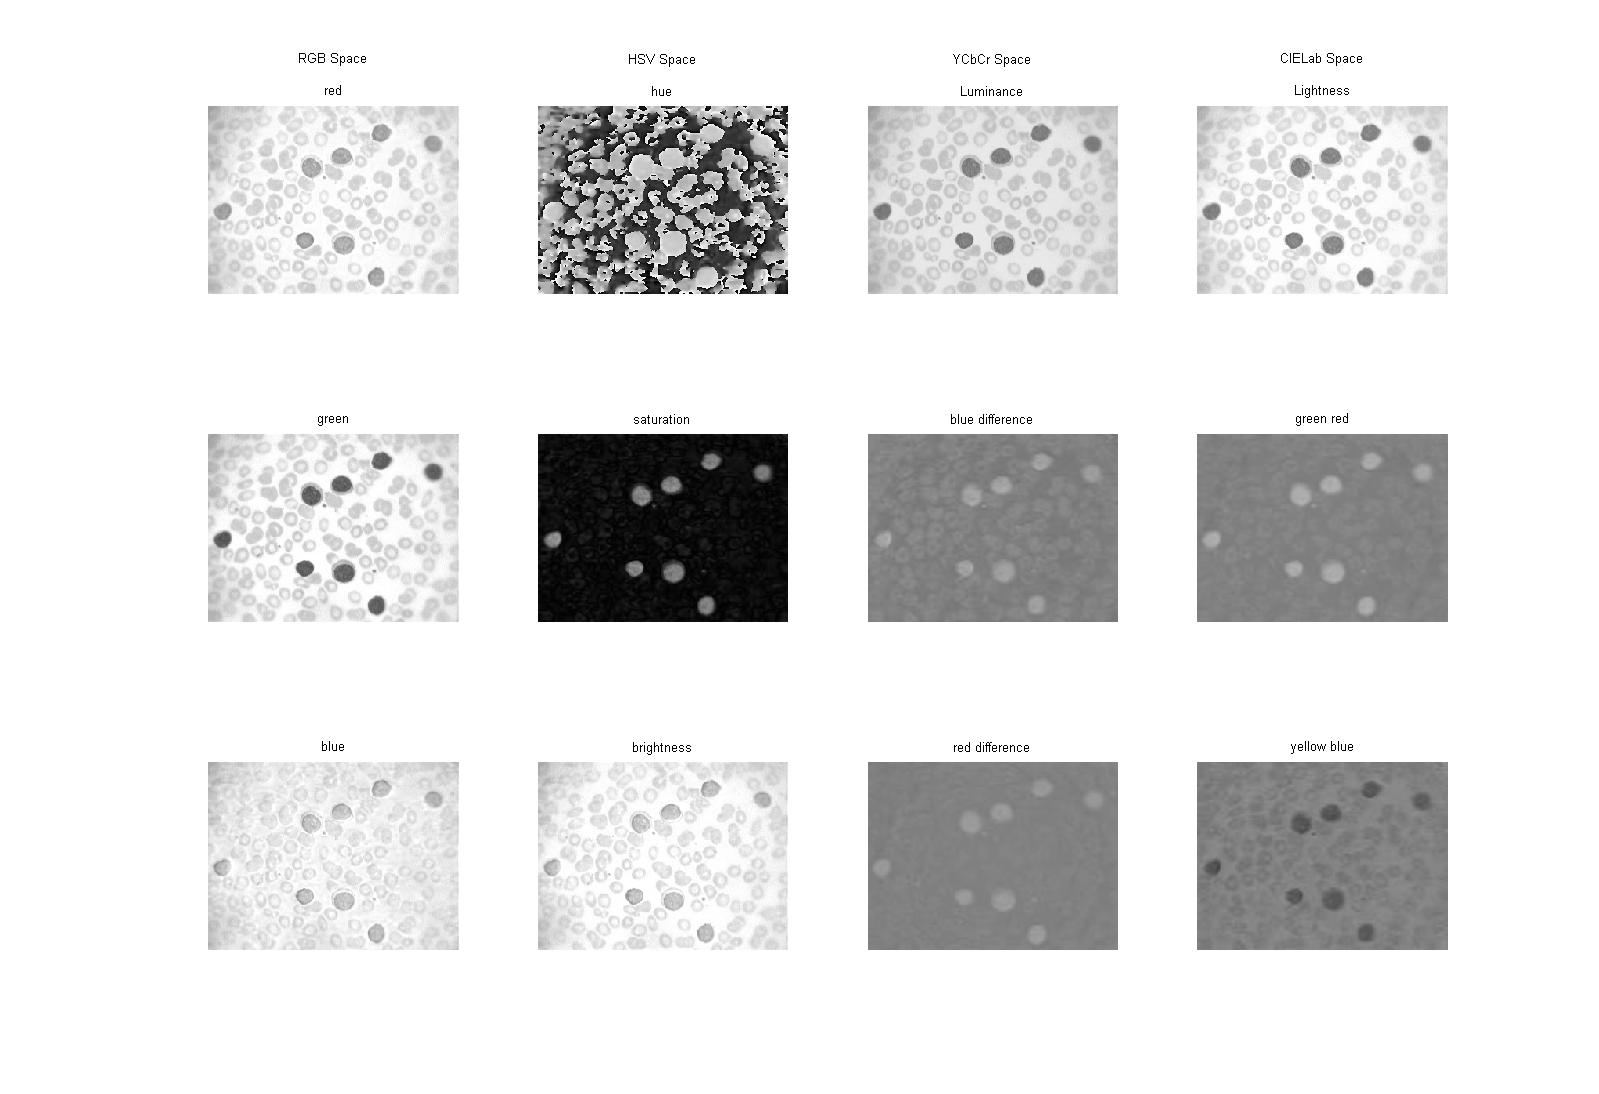
\includegraphics[width=\linewidth]{figure/Analysis/differences.jpg}
				\caption{Color space differences}
				\label{fig:differences}
			\end{figure}
		%Images from https://stackoverflow.com/questions/30022377/should-i-use-hsv-hsb-or-rgb-and-why
		Here we see that the leukocytes stand out the most in the saturation channel of the HSV color space. But they are also quite noticable in the green channel of RGB space. It would likely be the best option to use HSV in this case. 
		
			\subsubsection{Edge detection}
			
			Edge detection is performed by applying a variety of mathematical methods. Simply put, the algorithm will find points in a digital image in which the brightness changes abruptly. 
			
			\subsubsection{Blob detection}
			
			A BLOB, or "Binary Large OBject", refers to a group of connected pixels in a binary image. Detecting BLOBs in an image must be done before we can start analyzing and comparing their features. Examples of such features could be area, compactness, circularity, or center of mass.
			
			In order to make an image binary (each pixel being either completely black or completely white), a thresholding operation must be performed. The parameters of this function will greatly affect the resulting image to be processed. 
			
			Defining destinct BLOBs in a binary image is accomplished by going through the image one pixel at a time until a non-zero (foreground) pixel is found. One method is to now check the pixel's neighbors for connected foreground pixels, and so recursively check every neighbor's neighbor until the entire collection of pixels are assigned to the same object. This is called the grass-fire algorithm. Another method doesn't check recursively, instead requiring a second pass to correct certain BLOBs being classified as multiple objects.
			
			
			\subsubsection{Object recognition}
				Having extracted features from the detected objects, those features can be compared to those of pre-defined objects to determine if they match. A simple implementation might compare the color and circularity of an object to that of a perfectly round, red circle. 
				
				More advanced object recognition relies on deep learning algorithms, in which the program analyzes a digital catalog of object examples in order to define which paramaters best define a particular type of object.
			
		\subsection{Virtual Reality}
		The earliest attempts at a VR experience was in the 1950s\cite{VRS} by Morton Heilig who made the Sensorama\ref{fig:sensorama}; an arcade-style theater cabinet, that featured stereo speakers, stereoscopic 3D display, smell generators, fans and a vibrating chair.
		\begin{figure}[H]
			\centering
			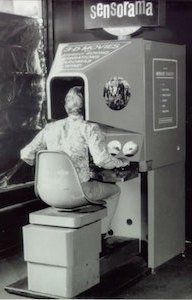
\includegraphics[width=0.4\linewidth]{figure/Analysis/sensorama2}
			\caption{The Sensorama made by Morton Heilig in the 1950s. Fully featured first step at virtual reality.}
			\label{fig:sensorama}
		\end{figure}
		There were a couple of short movies made for the Sensorama, but these were all produced and edited by Morton Heilig himself. The whole setup was stationary, and didn't feature any Head Mounted Display (HMD), so the user had to sit in the vibrating chair and look straight at the display for the duration of the movie. The more modern versions do not include features like smell and fans, but are also geared more towards mobility and full body immersion, and having a vibrating chair doesn't promote that idea.\\
		
		Morton Heilig later went on to further develop the idea of virtual reality, by making the first HMD in form of the Telesphere Mask\cite{VRS} in 1960. This took the immersive nature of his first product to a more personal level, even though it still just were a simple stereoscopic 3D wide view, with stereo sound. It did however look more like the virtual reality headsets of the modern day as seen in \autoref{fig:telesphere}.
		\begin{figure}[H]
			\centering
			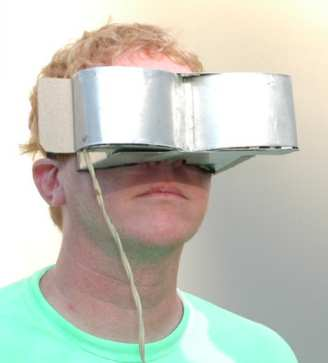
\includegraphics[width=0.25\linewidth]{figure/Analysis/TelesphereMask}
			\caption{The first attempt at HMD virtual reality headset, made by Morton Heilig in 1960. It worked by having stereoscopic 3D vision and stereo sound.}
			\label{fig:telesphere}
		\end{figure}
		Even though it was a step in the direction of a functioning virtual reality headset, it was still only a display showing a movie, it didn't have any motion tracking, or interaction between the user and the movie being watched. There was a sore lack of immersion, which is what makes the virtual reality headsets of today what they are.\\\\
		
		In 1961 the first motion tracking HMD was developed\cite{VRS}, it was made for military purposes, and was focused on tracking the head movements to control a remote camera. This was to allow a soldier to view remote locations in a natural fashion, without risking the viewer to actually be physically present. It used magnets to accomplish the head motion tracking.\\
		
		After the initial hype for virtual reality died down with the invent of the world wide web in the mid 90's, the industry waited patiently for hardware that could provide the immersion that tied the experience as a whole together. All of the early attempts had one flaw in common; the hardware couldn't provide close to realistic or good looking graphics at a frame rate that wouldn't induce motion sickness in the user, at a price that a normal consumer could afford\cite{vergeVR}. And hence the virtual reality industry laid dormant until 2013 when a certain Palmer Luckey, made a kickstarter for a virtual reality headset called Oculus Rift\cite{createOculus}. This headset kick started (No pun intended) the hype and interest in virtual reality as a medium.
		
		\subsubsection{Standalone VR}
		Oculus Go\footnote{Oculus Go: \url{https://www.oculus.com/go/}} is a virtual reality headset set to launch in the first quarter of 2018. Developed by the firm behind Oculus Rift, the Go shares many features with the Rift. It is designed for virtual reality games, social applications and different kinds of 360 degree experiences. Furthermore, the Go is lightweight with fabrics which increase comfort during long sessions. Unlike the Rift, Oculus Go does not need to be connected to a computer to function, enabling it to be used in new contexts such as outdoors and while traveling. It utilizes a simple controller for navigation and action to allow complex interaction within the featured applications, although it does not feature fully tracked motion control. Another strength the Go brings is the built in spatial audio, which alongside the 2560x1440 pixel display makes the Oculus Go a serious competitor to current mobile VR headsets.   \\
		\begin{figure}[H]
			\centering
			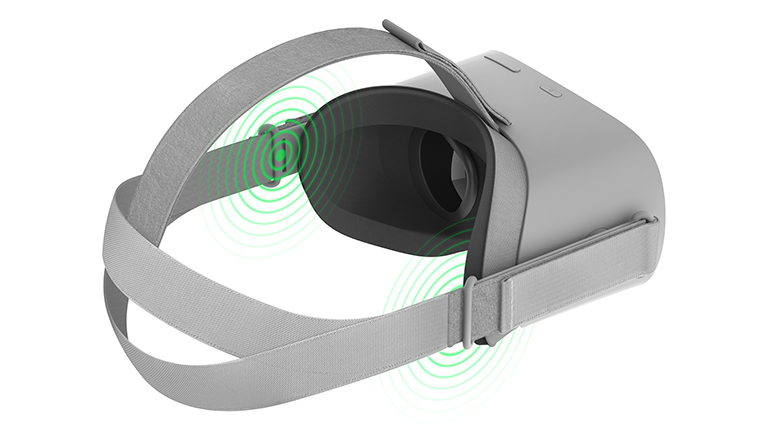
\includegraphics[width=1.0\linewidth]{figure/Analysis/oculusgo}
			\caption{The Oculus Go concept preview}
			\label{fig:Oculus}
		\end{figure}
		
		At the time this report is written, the product is not yet commercially available. Organizations developing for the headset may apply for an early version of the hardware to develop on. It is however possible to develop an application for the Go without owning one, as the Go is directly compatible with applications designed for GearVR. 
		
		Oculus Go is not the only standalone VR headset in the works. Google is working with Lenovo on Daydream, and HTC is developing the Vive Focus, a portable alternative to the HTC Vive. Little information is avaiable about the release date of either product, and the latter is set for a China-exclusive launch. As such, GearVR and Oculus Go are the only current options for portable VR development. \todo{do we need sources here?}
		
		
		\subsubsection{The essence of VR}
		Virtual reality is a medium\cite{definingVirtualReality}, a medium that has been a long time underway. Starting in the sixties, and being reborn in 2013 by Luckey Palmer, this medium is usually defined by a set of hardware implementations. These hardware implementations range a lot in price and devices, but a broad definition of the medium is:\\
		
		\begin{quote}
			\textit{Virtual Reality is electronic simulations of environments experienced via head-mounted eye goggles and wired clothing enabling the end user to interact in realistic three-dimensional situations}\cite{coates1992}.\\
		\end{quote}
		
		This definition is however quite old, being from 1992, but it does still apply to a certain degree to the current state of virtual reality as a device specific medium. Even though the devices, and their capabilities have changed, the way of interaction with the medium is largely the same; Put on a head mounted display, grab the controllers, and explore the 3D world you put yourself into. The rest of the paper will assume the definition of virtual reality as being:\\
		\begin{quote}
			\textit{Virtual Reality is electronic real time simulations of environments experienced via head-mounted eye goggles and one or more controllers enabling the end user to interact in realistic three-dimensional situations}\label{def:virtualRealityDefinition}.\\
		\end{quote}
		

    \section{State of the art}\label{sec:SOTA}
	  
		\subsection{VR Gardens}
			VR Gardens is a mobile application for designing and planning your own garden. It contains a variety of different 3D models of trees, bushes, outdoor furniture, tiles and the like, to help visualize any garden idea one might have. The design can then be reviewed using the Google Cardboard or similar simple Virtual Reality boxes to be immersed in a close-up edition of the design.
			\begin{figure}[H]
				\centering
				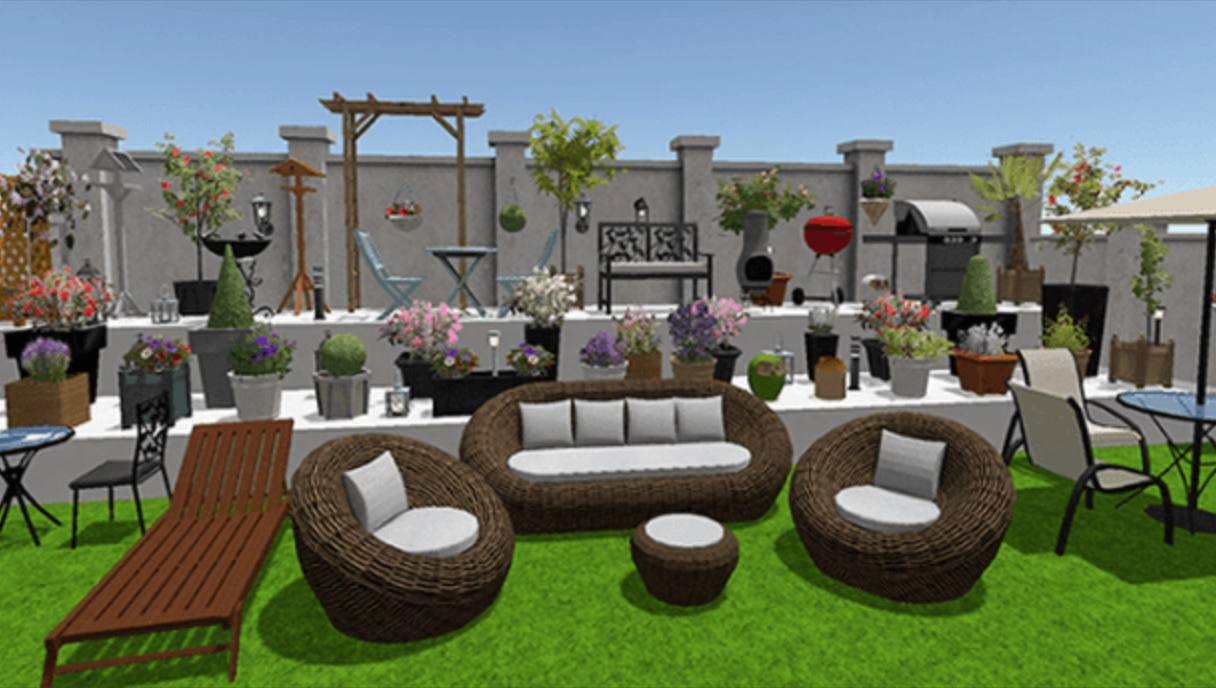
\includegraphics[width=0.6\linewidth]{figure/Analysis/vrgardens}
				\caption{VR Gardens comes with many pre-rendered 3D models}
				\label{fig:vrgardens}
			\end{figure}
			Although, because of the many functions of the application, it is also quite complex, and seems to have a rather steep learning curve. It is almost focused entirely on mobile as well, the web application implementation is just a ported version of the mobile application. Doing it exclusively on mobile is helping make it more mobile, but is also limiting the capabilities of both interface and hardware. The limited screen space has made the interface very compact and the controls feels clunky with touch. The effort can be noticed throughout the use, but ultimately the experience falls short due to the 	platform choice.
		\subsection{Mental Canvas}
			A software system that combines 2D draw-and-paint with 3D\footnote{Mental Canvas: \url{https://www.mentalcanvas.com}} which enables a user to create a 3D environment from sketches, supporting conceptual architectural design and analysis. It has been created for Microsoft's Surface technologies\footnote{Microsoft Surface: \url{https://www.microsoft.com/en-us/surface}} and is compatible with the Surface Dial. The system allows for the user to place 2D surfaces, or \textit{canvases} in a 3D space using traditional CAD(Computer-Aided Design) tools of positioning, scaling, rotating on XYZ-coordinate axes.\cite{sotaMentalCanvas}
			
				\begin{figure}[H]
					\centering
					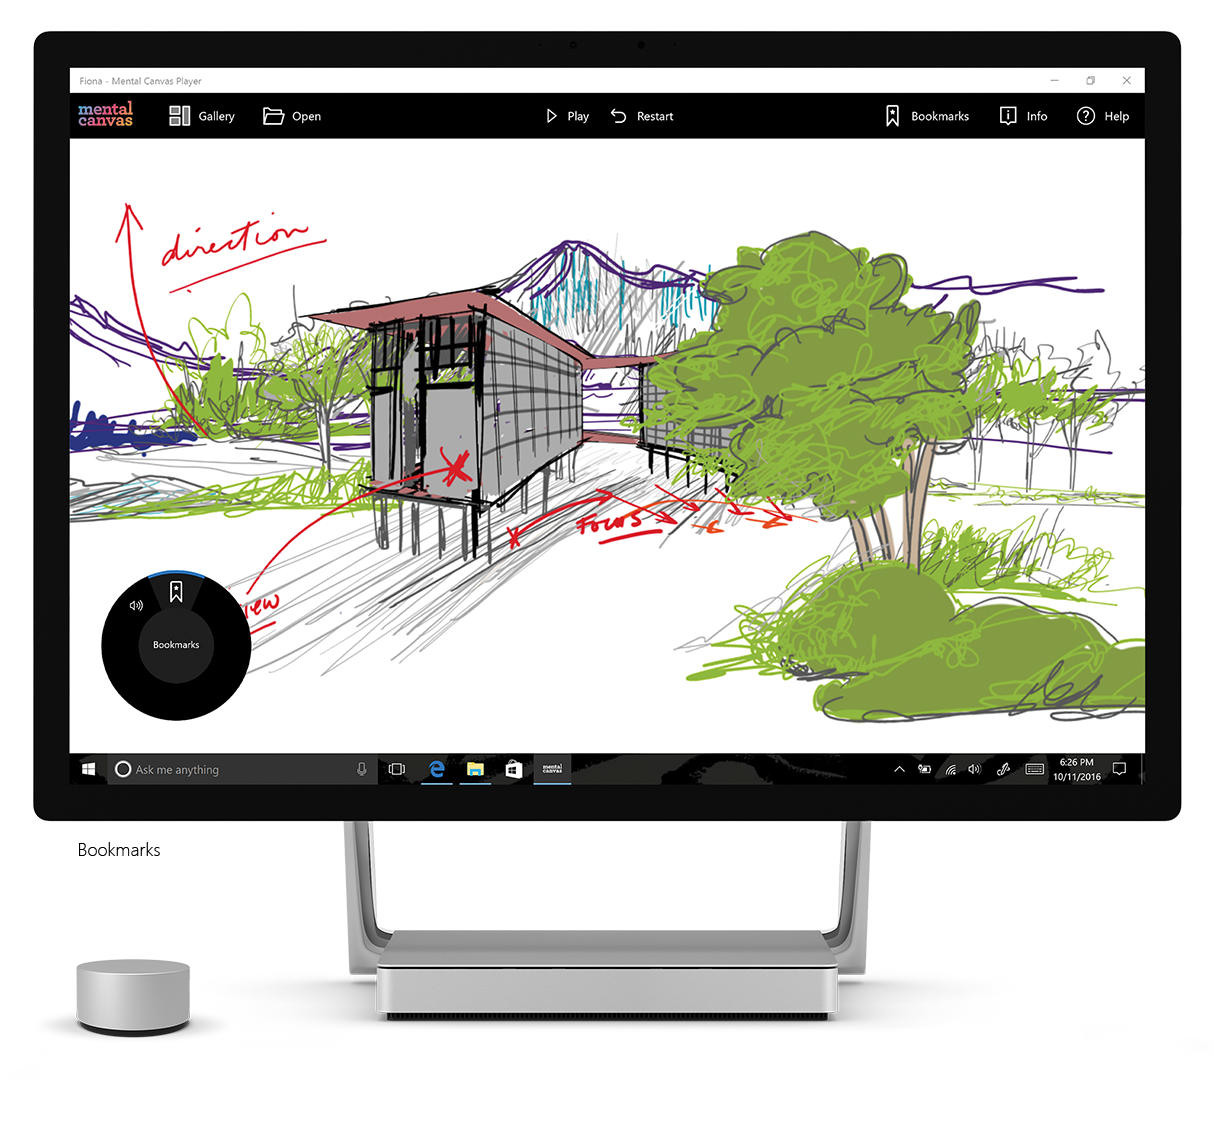
\includegraphics[width=0.5\linewidth]{figure/Analysis/mentalCanvas.png}
					\caption{Mental Canvas combines 2D sketching systems with 3D computer systems.}
					\label{fig:mentalCanvas}
				\end{figure}

		
		\subsection{Reactable}
			reacTIVision\footnote{reacTIVision: \url{http://reacTIVision.sourceforge.net/}} is a framework for developing computervision applications and interfaces. It uses fiducial markers as seen in  \autoref{sec:fiducialMarkers} to sense objects and movement, which allows for more extended interaction. \\
			
			Reactable\footnote{Reactable: \url{http://reactable.com/}} is a musical instrument that uses the reacTIVision framework, to map different controllers on a tabletop interface. The different types of fiducial markers displayed on cubes or small figures work as knobs, buttons and the like to imitate an analog synthesizer, but with different more visual interactions. It enhances the musician's or sound engineer's chance to be more visually creative with their music. The table itself consists of a camera at the bottom pointing upwards to the tabletop. The camera detects interactions made by the user and how the fiducial markers are altered, which results in a musical sound space.
				\begin{figure}[H]
					\centering
					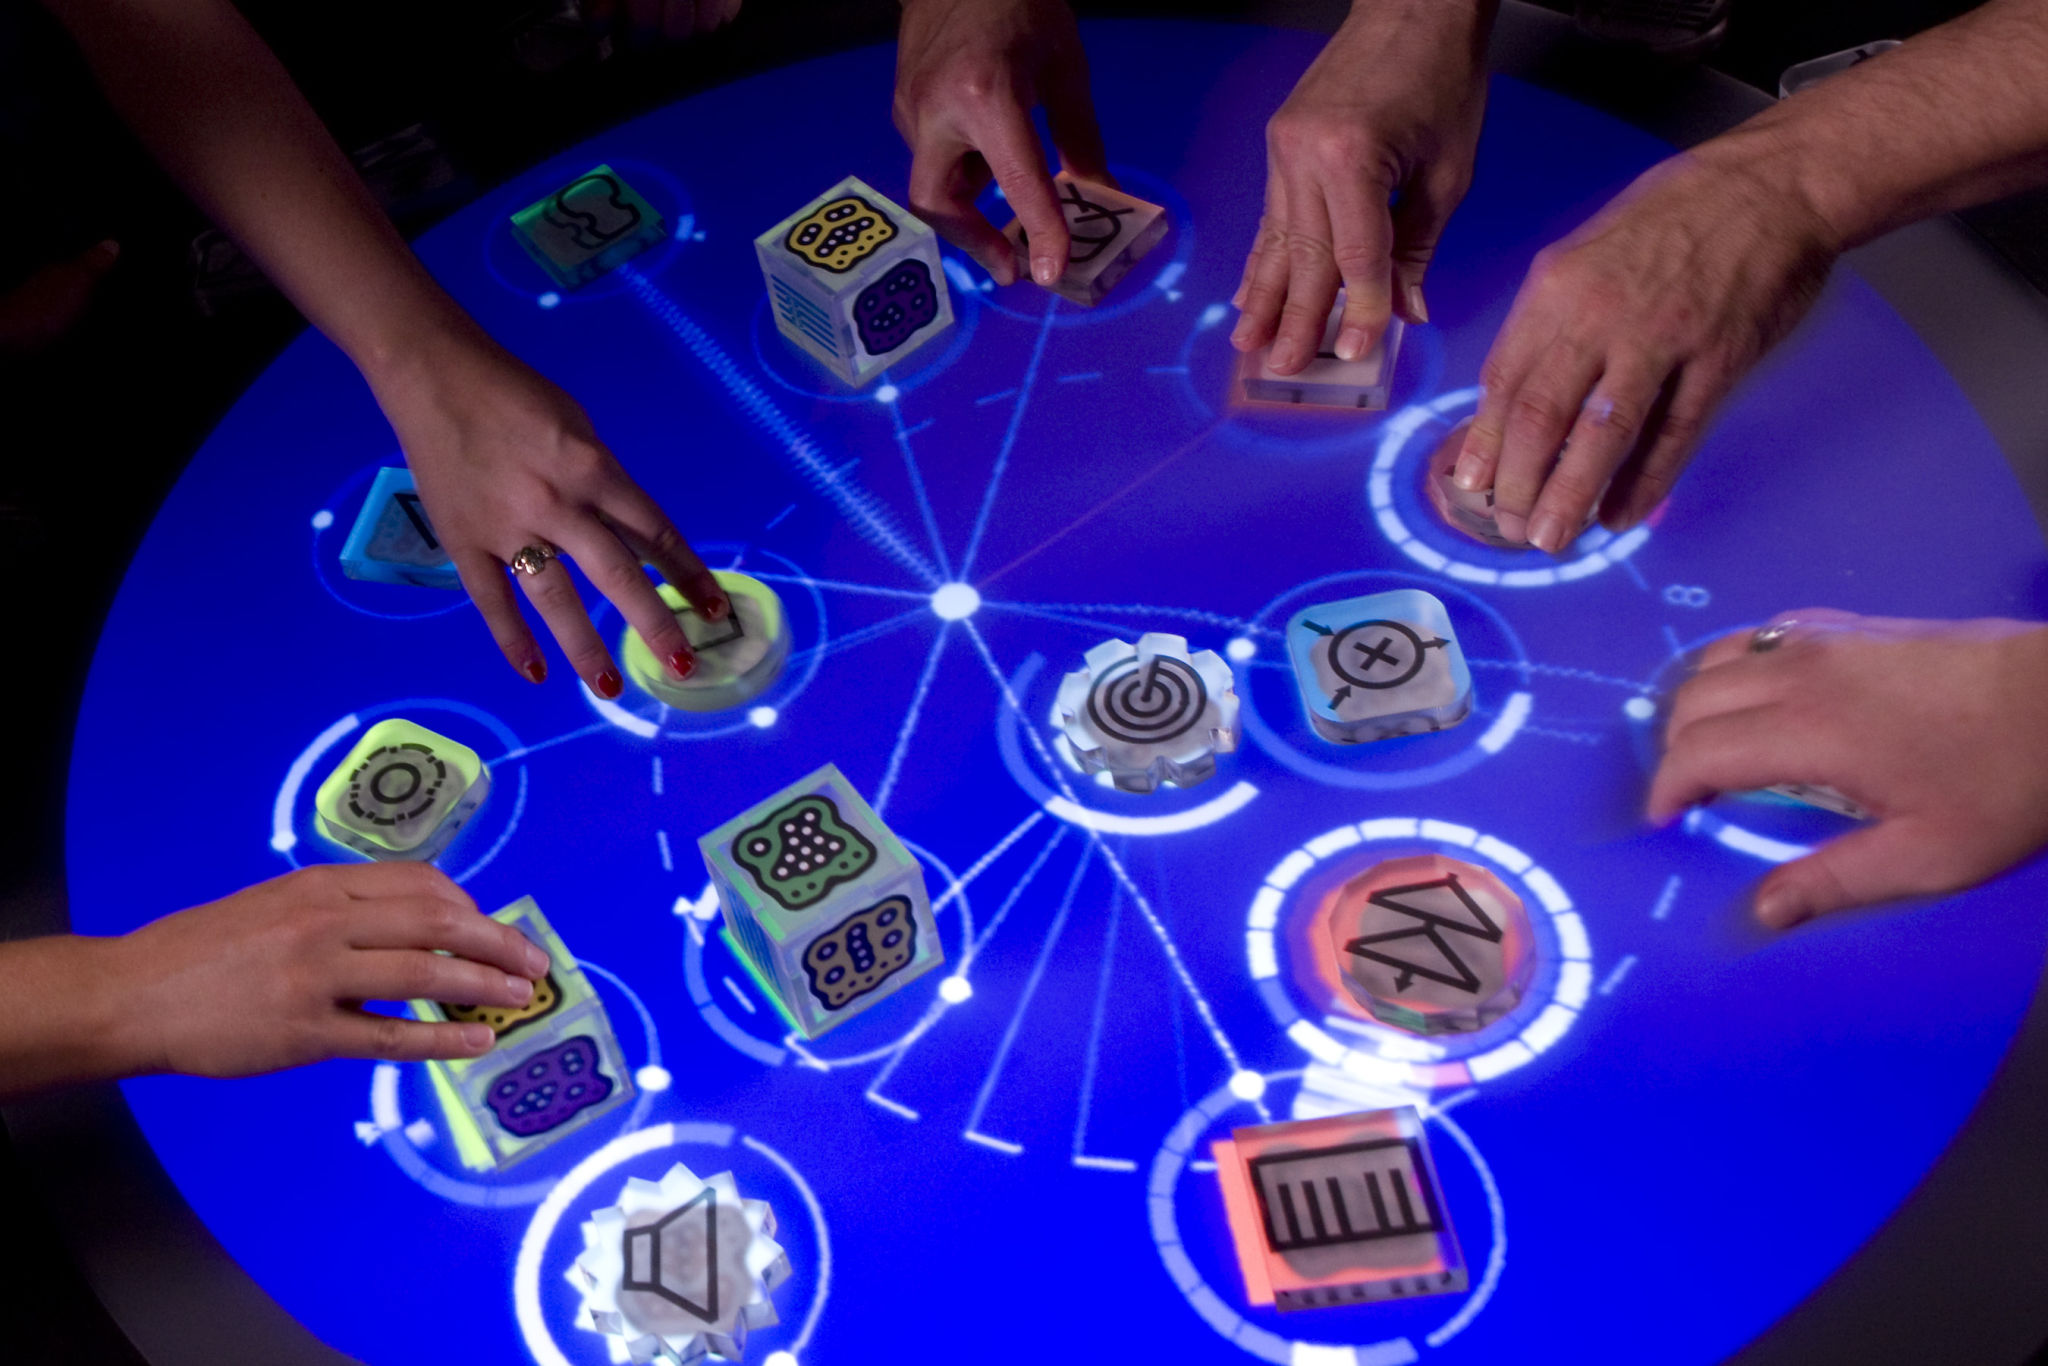
\includegraphics[width=0.6\linewidth]{figure/Analysis/reactable}
					\caption{The Reactable table synthesizer used by multiple users.}
					\label{fig:reactable}
				\end{figure} 
			
		
		\subsection{SketchUp}
			SketchUp\footnote{SketchUp: \url{https://www.sketchup.com/}} is a 3D modeling tool that allows for a user to create 2D lines and shapes, which can be manipulated through vertex editing turning it into 3D models in a simplistic fashion. When the 3D models are created SketchUp offers different functionalities for bringing details to the product, and then creating layout drawings from the final	model e.g. to show customers a house drawing or even landscape architecture. The software has it strengths and weaknesses in its simplicity, since it allows for intuitive modeling, but falls off on immersion making the designs seem stale. All though that could be seen as a weakness, it enables minimal memory usage to allow for a highly effortless experience. \\
			
			SketchUp exists in various versions for different professions like architecture, construction, engineering, landscape architecture and the like. Creators are enabled to share their models with the community, or save them for their own later use, to implement in bigger structure planning eg. a tree could be saved as an asset to use for a complete garden design.
			
				\begin{figure}[H]
					\centering
					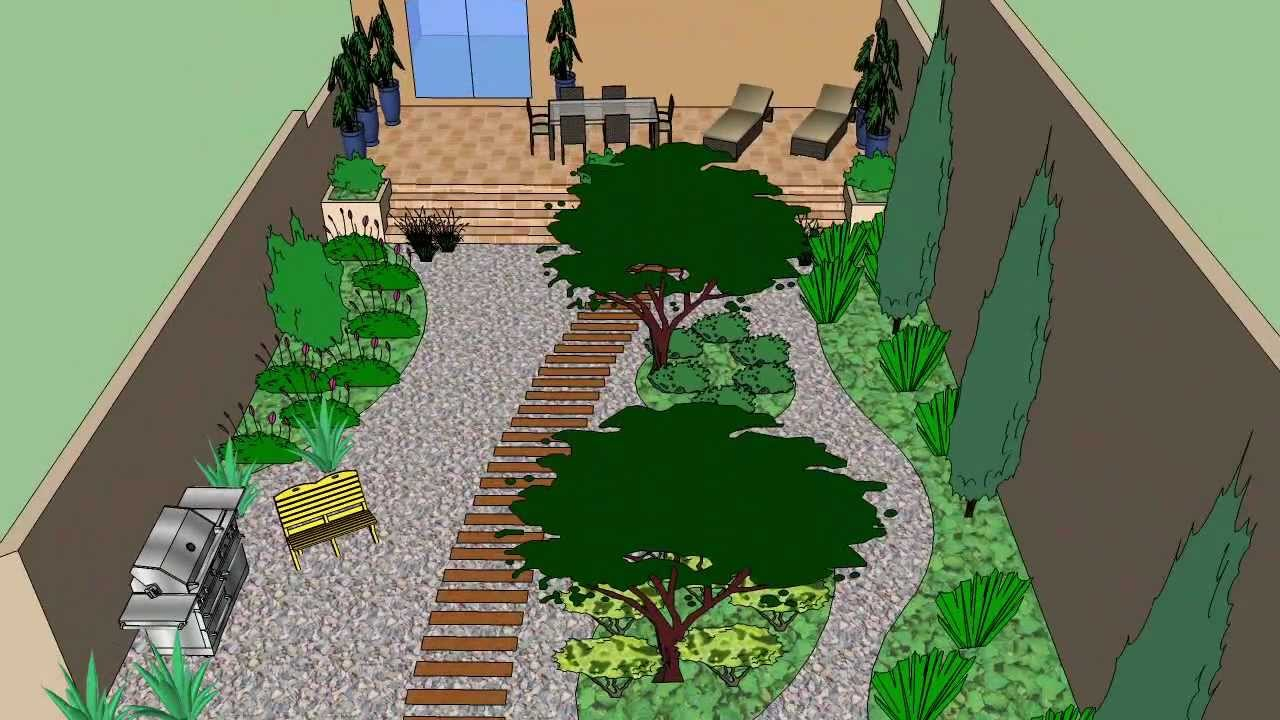
\includegraphics[width=0.6\linewidth]{figure/Analysis/sketchupgarden}
					\caption{A garden designed in SketchUp}
					\label{fig:sketchupgarden}
				\end{figure}
			
			\section{Design Requirements}
			%Some design requirements.
			I'm just going to vomit out some words here and hopefully get it sorted into correct categories before moving on to something else
			\begin{itemize}
			\item Must be able to add a reasonably large number of items to the garden without the program crashing
			\item Must be able to move tokens and have the virtual objects move with them in real time
			\item Virtual objects must not exhibit a noticable jitter
			\item Virtual object's position must correspond exactly to that of their physical token
			\item The application must include the most common plants found in a Danish garden in order to be functional
			\begin{itemize}
				\item Roses
				\item Rhododendron
				\item Apple trees
				\item Hydrangea
				\item Tulips
				\item Lilacs
				\item Strawberries
				\item Beech
				\item ... and more. How many? Who knows!
			\end{itemize}
			\item Rotation of token must rotate virtual object.
			\item (maybe?) Must be able to adjust size of virtual objects (how?)
			\item Object recognition may not fail more than x\% of the time.
			\item Physical construction of our prototype must be able to be easily taken apart and reconstructed, or simply be collapsible. Must also be lightweight. Otherwise we can't bring it anywhere yo
			\item Prototype must be able to function in most natural and artificial lighting conditions. It's okay if it can't operate in \textit{lightning} conditions... would be dope though.
			\item User must be able to walk around and look around in the virtual environment.
			\item Virtual environment must ideally run at like 90fps, but you know at LEAST 60fps or we're just being rude to the user.
			\item The program must run smoothly on a powerful laptop. (define smooth, define poweful)
			\item Environment should be pretty and detailed enough that it isn't distracting the user. 
			\item Program should be compatible with (Vive, GearVR, Rift... probably gon' be vive)
			\item Virtual garden should support garden sizes under 50 m$^2$ and like way over 800 m$^2$ because half our respondents had a garden larger than 800 m$^2$ so probably a good portion of them have gardens a lot bigger than that. Bastards.
			
			
			\end{itemize}
			
				\subsection{Functional requirements - TODO}
					What it should do\\
					\begin{itemize}
						\item It should be pleasurable to use by the end user.
						\item It should be useful, usable and accessible for the end user.
						\item It should not require a lot of effort from the end user to use.
						\item It should be easy to add objects to the virtual garden.
					\end{itemize}
					
				\subsection{Non-functional requirements - TODO}
					How it should do it\\
					\begin{itemize}
						\item It should incorporate physical, easy to distinguish tokens.
						\item It should make use of a virtual reality headset, to immerse the user.
					\end{itemize}
			